\chapter{Regla de independencia y prueba no clausal de teoremas}

En el presente capítulo se expondrá el diseño de un método de prueba de teoremas basado en la consistencia o inconsistencia del conjunto de fórmulas de partida, así como de la negación de la fórmula que se quiere deducir. En definitiva se basa en el hecho de que, si $K$ es una base de conocimiento y $F$ una fórmula proposicional:

$$K\vDash F \;\text{ si y sólo si }\; K \cup \{ \neg F \} \text{ es inconsistente}$$

La idea principal será hallar la inconsistencia del conjunto de fórmulas mediante la saturación de dicho conjunto en la constante $\bot$. Para saturar, se usarán las ya mencionadas retracciones conservativas,  que se calcularán mediante lo que se denominará un \textit{operador de omisión de variables}. \\

Este operador eliminará una de las variables cada vez que se aplique, obteniendo a cada paso un conjunto equivalente de fórmulas en los que se usa una variable menos. Finalmente, como hay un número finito de variables en $K \cup \{ \neg F \} $, llegará un momento en el que no queden variables y que sólo queden las constantes $\top$ o $\bot$ (sólo una de ellas), habiendo así refutado o probado, respectivamente, el teorema.\\

Un cambio relevante en la estructura de este capítulo respecto a la seguida en el capítulo anterior es que se expondrán en primer lugar las bases teóricas que fundamentan el modelo lógico-algebraico de razonamiento; y, posteriormente, se implementará en Haskell dicho modelo. 

\section{Retracción conservativa mediante omisión de variables}
En esta sección se presenta cómo calcular retracciones conservativas usando los ya mencionados operadores \textit{de omisión (o de olvido)}. Dichos operadores son mapas del tipo:
$$\delta : Form(\mathcal{L}) \times Form(\mathcal{L}) \longrightarrow Form(\mathcal{L}) $$
donde $2^X$ representa al conjunto potencia de $X$. 

\defn Sea $\delta$ un operador: $\delta :Form(\mathcal{L}) \times Form(\mathcal{L}) \longrightarrow Form(\mathcal{L} \setminus \{ p \})$  se dice que es:

\begin{enumerate}
\item \textit{robusto} si $\{F,G\} \vDash \delta (F,G)$.
\item un \textit{operador de omisión} para la variable $p \in \mathcal{L}$ si:
$$\delta (F,G) \equiv [\{F,G\}, \mathcal{L} \setminus \{p\}]$$
\end{enumerate} 

Una caracterización muy útil de los operadores se puede deducir de la siguiente propiedad semántica: Si  $\delta$ es un operador de omisión, los modelos de $\delta (F,G)$ son precisamente las \textit{proyecciones} de los modelos de $\{ F,G \}$ (ver figura \ref{fig:proy}). 

\vspace{0.5cm}
\begin{figure}[h]
	\centering
		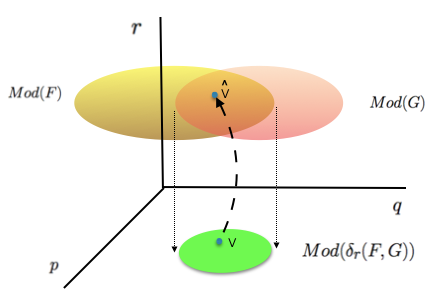
\includegraphics[scale=0.6]{imagenes/indemod.png}
	\caption{Interpretación semántica del operador de omisión (Lema de elevación)}
	\label{fig:proy}
\end{figure}
\vspace{0.5cm}

\lem \label{lem:lifting} (\textbf{Lema de elevación}) Sean $v :\mathcal{L} \setminus \{p\} \rightarrow \{ 0,1 \}$ una valoración o interpretación, $F, G \in Form(\mathcal{L})$ fórmulas y $\delta$ un operador de omisión de la variable $p$. Las siguientes condiciones son equivalentes:
\begin{enumerate}
\item $v \vDash \delta (F,G)$
\item Existe una valoración $\hat{v} : \mathcal{L} \rightarrow \{ 0,1 \}$ tal que $\hat{v} \vDash F \wedge G$ y $\hat{v} \upharpoonright_{\mathcal{L} \setminus \{ p \}} = v $
\end{enumerate}

\noindent \textbf{Prueba: } ($1 \Rightarrow 2$): Dada una valoración $v$, se considera la fórmula 
$$H_v = \bigwedge_{q \in \mathcal{L} \setminus \{ p \}} q^v$$
donde $q^v$ es $q$ si $v(q)=1$ y $\neg q$ en otro caso. Es claro que $v$ es la única valoración de $\mathcal{L} \setminus \{ p \}$ que es modelo de $H_v$. \\
Supongamos que existe $v  :\mathcal{L} \setminus \{p\} \rightarrow \{ 0,1 \}$ modelo de $\delta (F,G)$, pero que no se puede extender a un modelo de $F \wedge G$. Entonces la fórmula $$H_v \rightarrow \neg (F \wedge G)$$ es una tautología, en particular:
$$ \{ F,G \} \vDash H_v \rightarrow \neg (F \wedge G)$$
Como $ \{ F,G \} \vDash F \wedge G$, usando \textit{modus tollens} se tiene $\{ F,G \} \vDash \neg H_v$. Así que $\delta (F,G) \vDash \neg H_v$, por ser $\delta$ un retracción conservativa. Este hecho es una contradicción porque $v \vDash \delta (F,G) \wedge H_v$.\\
($2 \Rightarrow 1$): La extensión $\hat{v}$ verifica que:
$$\hat{v} \vDash F \wedge G \vDash [\{ F,G \} , \mathcal{L} \setminus \{ p \} ] \vDash \delta (F,G)$$
Como $\delta (F,G) \in Form(\mathcal{L} \setminus \{ p \})$, la valoración $v = \hat{v} \upharpoonright_{\mathcal{L} \setminus \{ p \}}$ también es modelo de $\delta (F,G)$. \hspace{14cm} $\square$ \\

En particular, el resultado es cierto para la propia retracción conservativa canónica $[K, \mathcal{L} \setminus \{ p \}]$, porque si consideramos la fórmula $\bigwedge K := \bigwedge_{F \in K} F$,
$$[K, \mathcal{L} \setminus \{ p \}] \equiv \delta_p (\bigwedge K , \bigwedge K)$$

Un caso interesante aparece cuando $\delta_p(F_1,F_2) \equiv \top$. En este caso, toda valoración parcial en $\mathcal{L} \setminus \{ p \}$ se puede extender a un modelo de $\{ F_1,F_2 \}$.\\

La siguiente caracterización será útil más adelante:
\cor Sea $\delta : Form(\mathcal{L}) \times Form(\mathcal{L}) \longrightarrow Form(\mathcal{L} \setminus \{ p \})$ un operador robusto. Las siguientes condiciones son equivalentes:
\begin{enumerate}
\item $\delta$ es un operador de omisión de la variable $p$.
\item Para cualesquiera $F,G \in Form(\mathcal{L})$ y $v \vDash \delta (F,G) $ valoración sobre $\mathcal{L} \setminus \{ p \}$, existe una extensión de $v$ modelo de $\{ F,G \}$.
\end{enumerate}

\noindent \textbf{Prueba:} ($1 \Rightarrow 2$): Cierta por el Lema de Elevación (Lema \ref{lem:lifting}).\\
($2 \Rightarrow 1$): Sean $F$ y $G$ dos fórmulas. Como $\delta$ es robusto, basta probar que:
$$\delta (F,G) \vDash [\{ F,G \}, \mathcal{L} \setminus \{ p \}]$$
Supongamos que no es cierto. En ese caso, existe una fórmula $H \in Form(\mathcal{L} \setminus \{ p \})$ tal que $[\{ F,G \}, \mathcal{L} \setminus \{ p \}] \vDash H$ (luego $H$ también es consecuencia lógica de $\{ F,G \}$), pero existe una valoración $v$ que satisface $v \vDash \delta (F,G) \wedge \neg H$. Por $(2)$, existe $\hat{v}$ extensión de $v$ que es modelo de $\{ F,G \}$. Por tanto, $\{ F,G \} \vDash \neg H$, lo que es una contradicción. \hspace{7.7cm} $\square$ \\

\cor Si $p \notin var(F)$, y $\delta_p$ es un operador de omisión de $p$, entonces
$$\delta_p(F,F) \equiv F \;\;\;\;\;\;\;\; \text{y} \;\;\;\;\;\;\;\; \delta_p (F,G) \equiv \{ F,\delta_p (G,G) \}$$

\noindent \label{cor:pnotinvar} \textbf{Prueba:} Si $p \notin var(F)$, entonces $\{ F \} \equiv [\{ F \} ,\mathcal{L} \setminus \{ p \}] \equiv \delta_p (F,F)$.\\
Por otro lado, $\delta_p (F,G) \equiv [\{ F,G \} , \mathcal{L} \setminus \{ p \}] \vDash \{ F,\delta_p (G,G) \}$. Para probar que en realidad se trata de una equivalencia se mostrara que tienen los mismos modelos.\\
Sea $v$ una valoración sobre $\mathcal{L} \setminus \{ p \}$ tal que $v \vDash \{ F,\delta_p (G,G) \}$. Entonces existe $\hat{v}$ (una extensión de $v$) tal que $\hat{v} \vDash G$. Como $\hat{v} \vDash F$ se tiene por el Lema de Elevación que $v \vDash \delta (F,G)$. \hspace{14cm} $\square$ 
 
\subsubsection{Retracciones conservativas inducidas por un operador de omisión} 
 
En el artículo \cite{Lang2003} J. Lang et al.  presentan un método de omisión de $X$ (un conjunto de variables de la fórmula $F$), denotado por $\texttt{forget}(F,X)$ y basado en la construcción de disyunciones de la siguiente forma:\\

\begin{tabular}{lll}
$\texttt{forget}(F, \emptyset)$ & $=$ & $F$\\
$\texttt{forget}(F, \{ x \})$ & $= $ & $F\{x/\top \} \cup F\{x/\bot \}$ \\
$\texttt{forget}(F, \{ x \} \cup Y)$ & $= $ & $\texttt{forget} (\texttt{forget}(F,Y),\{ x \})$
\end{tabular}

\vspace{0.5cm}

Notar que con este método el tamaño de $\texttt{forget}(F,Y)$ puede ser realmente grande. En el método que se expone en el trabajo se pretende simplificar la representación mediante el uso de operaciones algebraicas sobre proyecciones polinomiales.\\

Tal y como se ha descrito anteriormente, el operador de omisión de la variable $p$ actúa entre pares de fórmulas. A continuación, se extenderá la definición del operador de forma que se pueda aplicar a conjuntos de fórmulas o bases de conocimiento.

\defn Sea $\delta_p$ un operador de omisión de la variable $p$ y $K$ una base de conocimiento. Se define $\delta_p [\cdot ]$ como:\\

\begin{tabular}{l}
$\delta_p [\cdot ] : 2^{Form(\mathcal{L})} \rightarrow 2^{Form(\mathcal{L})}$ \\
$\delta_p [K] := \{ \delta_p (F,G) : F,G \in K \}$
\end{tabular}

\vspace{0.5cm}

Si se supone que se tiene un operador de omisión $\delta_p$ para cada $p\in \mathcal{L}$:

\defn Se llamará \textit{saturación} de la base de conocimiento $K$ al proceso de aplicar los operadores $\delta_p [\cdot ]$ (en algún orden) respecto a todas las variables proposicionales de $\mathcal{L}(K)$, denotando al resultado como $sat_{\delta}(K)$ (el cual será un subconjunto de $\{ \top , \bot \}$).\\

Posteriormente se verá que $sat_{\delta}(K)$ no depende del orden de aplicación de los operadores. Además, se probará que debido a que los operadores de omisión son robustos, si $K$ es consistente entonces necesariamente $sat_{\delta}(K)=\{ \top \}$.\\

A partir de los operadores de omisión resulta natural definir el siguiente cálculo lógico:

\defn Sea $K$ una base de conocimiento, $F\in Form(\mathcal{L})$ y $\{ \delta_p : p \in \mathcal{L}(K) \}$ una familia de operadores de omisión.
\begin{itemize}
\item[•] $A \vdash_{\delta}$-prueba en $K$ es una secuencia de fórmula $F_1, \dots ,F_n$ tal que para todo $i \leq n$, $F_i \in K$ ó existen $F_j , F_k (j,k < i)$ tal que $F_i = \delta_p (F_j , F_k)$ para algún $p \in \mathcal{L}$.
\item[•] $K \vdash_{\delta} F$ si existe una $\vdash_{\delta}$-prueba en $K$, $F_1, \dots ,F_n$, con $F_n = F$.
\item[•] Una $\vdash_{\delta}$-refutación es una $\vdash_{\delta}$-prueba de $\bot$.
\end{itemize}

La completitud (refutacional) del cálculo asociado a los operadores de omisión se enuncia como sigue:

\thm \label{teo:completo} Sea $\{ \delta_p : p \in \mathcal{L} \}$ una familia de operadores de omisión. Entonces $\vdash_{\delta}$ es refutacionalmente completo, es decir, $K$ es inconsistente si y sólo si $K \vdash_{\delta} \bot$.\\

\noindent \textbf{Prueba:} La idea es saturar la base de conocimiento como en la Figura (\ref{fig:comple}). Si $sat_{\delta} (K) = \{ \top \}$, entonces, aplicando repetidas veces el lema de elevación, se puede extender la valoración vacía (la cual es modelo de $\{ \top \}$) a un modelo de $K$.\\
Si $\bot \in sat_{\delta} (K)$ entonces $K$ es inconsistente, porque $K \vDash sat_{\delta} (K)$ por robustez de los operadores de omisión. $\square$ %% La elección de una $\vdash_{\delta}$-refutación en particular es sencilla.

\vspace{0.5cm}
\begin{figure}[h]
	\centering
		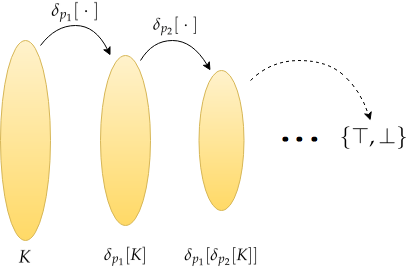
\includegraphics[scale=0.44]{imagenes/comple.png}
	\caption{Decidir la consistencia usando operadores de omisión ($\partial_{p_i}$)}
	\label{fig:comple}
\end{figure}
\vspace{0.5cm}

\cor \label{cor:omitep} $\delta_p [K] \equiv [K, \mathcal{L} \setminus \{ p \}]$

\noindent \textbf{Prueba:} Por robustez del operador de omisión $\delta_p$ se tiene:
$$[K, \mathcal{L} \setminus \{ p \}] \vDash \delta_p [K]$$

Para probar la otra dirección, se considera $F\in [K, \mathcal{L} \setminus \{ p \}]$ y se supone que $\delta_p [K] \nvDash F$. Entonces $\delta_p [K] + \{ \neg F \}$ es consistente. En particular, si se satura se tiene: $sat_{\delta}(\delta_p [K] \cup \{ \neg F \}) = \{ \top \}$.\\
Como $p \notin var(\neg F)$ se puede usar el corolario \ref{cor:pnotinvar}, obteniendo que para todo $G\in K$:
$$\delta_g (\neg F, G) \equiv \{ \neg F, \delta_g  (G,G)  \} \;\;\;\;\;\;\;\;\;\;\;\; \text{y} \;\;\;\;\;\;\;\;\;\;\;\; \delta_p (\neg F , \neg F) \equiv \neg F$$
Por consiguiente,
$$\delta_p [K \cup \{ \neg F \}] \equiv \delta_p [K] \cup \{ \neg F \}$$
así que, aplicando saturación empezando por $p$:
$$sat_{\delta}(K \cup \{ \neg F \}) \equiv sat_{\delta}(\delta_p [K] \cup \{ \neg F \})$$
Lo que indica que $K \cup \{ \neg F \}$ es consistente, luego $K \nvDash F$, que es una contradicción. $\square$\\

Dados $Q \subseteq \mathcal{L}$ y un orden lineal $q_1 < \cdots < q_k$ sobre $Q$, se define el operador: $$\delta_{Q,<} := \delta_{q_1} \circ \cdots \circ \delta_{q_k}$$

Este, no es más que la aplicación sucesiva del operador de omisión $\delta$  respecto de cada una de las variables de $Q$ en un orden dado. De hecho, si prescindimos de hacer explícito el orden, el operador está bien definido módulo equivalencia lógica. En otras palabras, dados dos órdenes sobre $Q$ cualesquiera, producen bases de conocimiento equivalentes. Esto es cierto puesto que para cada $p,q \in \mathcal{L}$, usando el corolario \ref{cor:omitep} se sigue que:
$$ \delta_p \circ \delta_q [K] \equiv \delta_q \circ \delta_p [K]$$
\noindent ya que ambas son equivalentes a $[K, \mathcal{L} \setminus \{ p,q \}]$. Por consiguiente y con la idea de simplificar la notación, se escribirá $\delta_Q$ cuando no importe la presentación sintáctica de dicha base de conocimiento.\\

Como consecuencia del teorema \ref{teo:completo} y el corolario \ref{cor:omitep} se da que el hecho de saber si una fórmula es o no consecuencia lógica de otra (o de una base de conocimiento) se puede reducir a otro problema similar en el que sólo se trabaje con las variables de la fórmula objetivo. Basta con eliminar de forma sucesiva todas las variables de la base de conocimiento que no ocurran en la fórmula objetivo. A esta propiedad se le conoce como \textit{Propiedad de localización}:

\cor (\textbf{Propiedad de Localización \cite{Borrego2009}}) Las siguientes condiciones son equivalentes:
\begin{enumerate}
\item $K \vDash F$
\item $\delta_{\mathcal{L} \setminus var(F)} [K] \vDash F$
\end{enumerate}

\noindent \textbf{Prueba:} Trivial, porque $\delta_{\mathcal{L} \setminus var(F)} [K] \equiv [K,var(F)]$

\section{Derivadas Booleanas}
Con el objetivo de definir el operador de omisión que se usará en la herramienta, se hará uso de las derivadas polinomiales aunque no de forma directa. En la práctica, se traducirá la derivada sobre $\mathbb{F}_2 [\textbf{x}]$ tradicional a un operador sobre fórmulas proposicionales.\\

Antes de continuar se expondrán diversas propiedades básicas. Recalcar que una derivación sobre un anillo $R$ es una mapa $d:R \rightarrow R$ verificando que $\forall a,b \in R$:

\begin{itemize}
\item[•] $d(a+b) = d(a) + d(b)$
\item[•] $d(a \cdot b) = d(a) \cdot b + a \cdot d(b)$
\end{itemize}

La traducción al mundo de la lógica de las derivaciones se construye tal y como sigue:

\defn \cite{Borrego2009} Un mapa $\partial : Form(\mathcal{L}) \rightarrow Form(\mathcal{L})$ es una \textit{derivada Booleana} si existe una derivación $d$ sobre $\mathbb{F}_2 [\textbf{x}]$ tal que el siguiente diagrama sea conmutativo:

\begin{table}[h]
\centering
\begin{tabular}{ccc}
 $Form(\mathcal{L})$& $\xrightarrow{\partial} $ & $Form(\mathcal{L})$ \\ \\
 $\pi \; \downarrow $ & $\#$ & $\uparrow \Theta$ \\\\
 $\mathbb{F}_2 [\textbf{x}]$ & $\xrightarrow{d}$ & $\mathbb{F}_2 [\textbf{x}]$
\end{tabular}
\end{table}
 
 \noindent O lo que es lo mismo: $$\partial = \Theta \circ d \circ \pi $$
 
 En este trabajo, la atención recae sobre una derivada booleana en particular, denotada por $\frac{\partial}{\partial p}$, e inducida por la derivada $d = \frac{\partial}{\partial x_p}$. El siguiente resultado muestra una expresión semánticamente equivalente de esta derivada:
\prop $\frac{\partial}{\partial x_p} F \equiv \neg (F\{ p/\neg p \} \leftrightarrow F) $

\noindent \textbf{Prueba:} Es fácil ver que
$$\pi (F\{ p/\neg p \}) (x) = \pi (F) (x_1, \dots , x_p +1 ,\dots , x_n)$$
\noindent Por otro lado, se cumple que para fórmulas polinomiales:
$$\frac{\partial}{\partial x}a(x) = a(x+1)+a(x)$$
\noindent Así que,
$$\frac{\partial}{\partial x_p} \pi (F) = \pi (F) (x_1, \dots , x_p +1 ,\dots , x_n) + \pi (F) (x_1, \dots , x_n)$$
\noindent Y por tanto, aplicando $\Theta$ se tiene
$$\frac{\partial}{\partial p} F = \Theta (\frac{\partial}{\partial x_p} \, \pi (F)) \equiv \neg (F\{ p/\neg p \} \leftrightarrow F)$$
\hspace{15cm} $\square$ \\

Notar que el valor de verdad de $\frac{\partial}{\partial p}F$ respecto de una valoración no depende del valor de verdad de la propia $p$, luego se pueden aplicar valoraciones sobre $\mathcal{L} \setminus \{ p \}$ a dicha fórmula. De hecho, se puede describir la estructura de $F$ aislando el rol de la variable $p$ de la siguiente manera:

\lem \cite{Borrego2009} (Forma $p$-normal) Sea $F \in Form(\mathcal{L})$ y sea $p$ una variable proposicional.

\section{Regla de independencia}

\section{Cálculo lógico}